\documentclass[10pt,conference,compsocconf]{IEEEtran}

%\usepackage{times}
%\usepackage{balance}
\usepackage{url}
\usepackage{graphicx}	% For figure environment

\usepackage{booktabs}
\usepackage{amsmath,amssymb}
\usepackage{xcolor}
\newcommand\TODO[1]{\textcolor{red}{#1}} % for all TODOs
\usepackage{pdfpages}

\begin{document}
\title{Computational Intelligence Lab Report\\ {\large Galaxy Image Generation}}

\author{Sven Kellenberger, Hannes Pfammatter, Till Schnabel & Michelle Woon \\group: Galaxy Crusaders, Department of Computer Science, ETH Zurich, Switzerland}

\maketitle

\begin{abstract}
This paper explores various ways for generating as well as approximating a similarity function for high resolution cosmology images. The methods solving the latter issue is evaluated via Kaggle\cite{Kaggle}, achieving 2nd place on the public leaderboard.

For the similarity score approximator, an advanced Random Forest (RF) method is evaluated and compared to a Convolutional Neural Network (CNN) and a simpler RF approach. The structure of our CNN will be introduced and analyzed. This paper also provides insights to the advanced RF used, such as how and why it performed better than the CNN. We will also discuss the image preprocessing and data augmentation used for all learning methods introduced in this paper. 

For the generation of the highly space cosmology images, an adhoc method, a Variational Autoencoder (VAE), a conditional Deep Convolutional Generative Adversarial Network (cDCGAN) and also a PixelCNN \TODO{(leave this?)} approach are all explored. We will discuss and evaluate each method in this paper. We present our cDCGAN on k-means clustered stars method.
\end{abstract}

\section{Introduction}
\label{sec:introduction}
Similarity scorers are useful for finding similar images to a given image. In this paper we evaluate RFs and a CNN as approximators of a similarity function for a cosmology image. The simpler RF does not make use of FFT, while the advanced RF and the CNN approximators use it. Despite being the more "sophisticated" method of the two advanced methods, the CNN performs worse in both time and mean absolute deviation. Our advanced RF approximator reaches a mean absolute deviation of 0.09542 on the public and 0.10463 on the private test set, scoring slightly better than the CNN.

Image generation is not a novel problem, however the task to generate sparse high resolution data has proven to be difficult for generative models. Hence, to solve this issue for generating cosmology images, we split the task into the generation of small $28\times28$ patches of single stars only, extracted from the given galaxy images, and the distribution of the results on a plain high resolution background image. We keep the distribution close to the given data.

%%%%%%%%% TODO
\TODO{Mention the best generator. (cDCGAN?)}
%%%%%%%%%

\TODO{Related work is not in the guideline, but I guess they add them in "Models and Methods"}
\section{Related Work}
To prevent overfitting, Srivastava et al.\@ \cite{Dropout} introduced Dropout in 2014. The idea is that e.g.\@ a fully connected layer is followed by such a dropout layer that sets a configurable percentage of output neurons to zero during training, thus effectively omitting their impact on the final output. Consequently, the preceding layer is less likely to overfit to training data, because it is forced to learn a more meaningful representation of the data using all neurons.

In 2015, Ioffe et al.\@ \cite{BatchNorm} introduced BatchNorm --- a normalization technique that takes as input the batch of data and normalizes across this batch. Other than for instance normalization during pre-processing, a BatchNorm layer contains learnable mean and variance, s.t.\@ the network may adjust to covariate shifts and vanishing gradients in between layers. Today, it is widely used in classification and other networks, to speed up the learning process.

Also in 2015, He et al.\@ \cite{ResNet} released their ResNet architecture, which uses so-called ``Skip connections'' that allow for far deeper architectures than practical ones before. The output of a building block of a few convolutional layers is summed with this block's original input, which allows the network to skip unwanted blocks. This process, they call ``Residual learning''. The problems of deep architectures like zero gradients were compensated by this new invention.

\section{Models and Methods}
\TODO{TODO: For all approaches: model and method as described in the help pdf that the course provides}

\subsection{Data}
We used the scored images to learn the similarity function. To train our models, we either used the labeled images only or the labeled images and a fraction of the scored images. This is because as we focused on stars, the labeled images provided enough data.

The data used from this project was downloaded from the Kaggle competition \cite{Kaggle}. It comes with 3 different sets of images:
\begin{itemize}
    \item Labeled: The images in this set are labeled on whether they are cosmology images or not.
    \item Scored: The images in this set are scored from 0 to 8 on their similarity to a prototypical cosmology image. A score like 2.61 means that the image almost coincides with said prototype. The higher the score the more similar the image is.
    \item Query: Images to assign scores to for the competition.
\end{itemize}


\subsection{Similarity Function Approximators}
\subsubsection{Simple Random Forest (SRF)} % easy baseline
\TODO{TODO}

\subsubsection{Advanced Random Forest (ARF)} % novel solution
\TODO{TODO}

\subsubsection{CNN} % hard baseline
%%%%%% Add an image of the CNN model
For the neural network approach for image classification, we used a deep convolutional architecture. We experimented a lot with the specific layers. Most experiments were performed on lower-resolution images ($125\times125$ and $250\times250$), because simple patterns like the star distribution could similarly be captures on this resolution while saving lots of computation time. Good settings were then applied to the original data. Our most important discoveries were:
\begin{itemize}
    \item Batch normalization greatly stabilizes and thus accelerates the training.
    \item Because the final score is linear between 0 and 8, a sigmoid layer times 8 in the end makes it harder for the network to predict the score correctly and is thus counter beneficial.
    \item A fast fourier transform (FFT) improves and stabilizes the training.
    \item Many convolutions but few parameters lead to the best results, because more convolutions mean a greater receptive field and a lot of parameters quickly cause overfitting on the sparse images.
    \TODO{Residual connections did not help?}
\end{itemize}
Our final architecture can be seen in figure \ref{fig:nn_classifier_arch}.  Not mentioned is the padder that pads the intermediate code from $125\times125$ to $128\times128$ spatial resolution. The number of features were raised by a factor of 2 every stacked convolutional block (colored in blue) until the maximum of 32 was reached. In total, there were eight of these blocks. No bias was used. The network had a total of only 37,376 parameters, 37,120 of which trainable. We reached a score of 0.16792 on the public and 0.18781 on the private part of the test set, after training the model for 140 epochs.
\begin{figure}
    \centering
    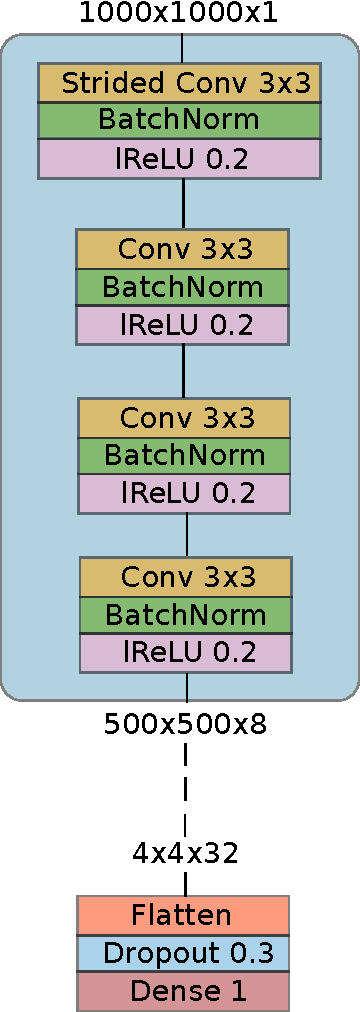
\includegraphics[width=0.4\columnwidth]{assets/nn_classifier_arch.pdf}
    \caption{Illustration of the CNN classifier architecture.}
    \label{fig:nn_classifier_arch}
\end{figure}

\subsection{Generators}
\subsubsection{Adhoc Generator (AG)} % easy baseline

\TODO{TODO: why this works}

Using the available labelled data, we detect stars in all the cosmology images by finding contours in the image. Doing this also allows us to find the minimum and maximum amount of stars in a cosmology image. 

Each image to generate first starts out as a black destination image. Then, for each image to generate a random number between the minimum and maximum amount of stars is selected. For each star to place into the image, a random source cosmology image is chosen and then a random star from that source image is taken. That star is then placed on a random spot in the destination image.

\subsubsection{DCGAN}
Data preprocessing. The pixel intensities are normalized to the range [-1, 1]. This is due to the output layer of the generator network using a tanh activation function. Further, the images are padded to size 1024 x 1024 which simplifies downsampling and upsampling. Model specification. Goodfellow et al. \cite{NIPS2014_5423}. Radford et al. provide a collection of hyperparameters. Their original implementation can be found online. Various improvements are available. Our main change to the DCGAN architecture was to follow (cite) and use nearest neighbor interpolation instead of transposed convolution for upsampling. Because the DCGAN architecture stabilizes training it was used. It was scaled up to be able to generate 1000 x 1000 images. Method specification. Figure I shows the architecture of the generator and the discriminator networks. Maybe add 28x28 images of stars which do not look well. 
\TODO{TODO}
\subsubsection{Star VAE} % hard baseline
In this section, the variational autoencoder (VAE) which is used to generate images of stars is described. \\
The variational autoencoder was introduced in 2014 by Kingma and Welling \cite{DBLP:journals/corr/KingmaW13}. Our implementation is based on the original paper as well as on the tutorial on variational autoencoders by Doersch \cite{doersch2016tutorial} and on a reference implementation on the TensorFlow website \cite{cvaetf}. \\
The VAE allows to encode data points to low-dimensional latent representations  $\sim\mathcal{N}(0, I)$ and to generate new data points by decoding arbitrary latent vectors $\sim\mathcal{N}(0, I)$. This is achieved by learning to map each data point x to a Gaussian distribution $q_{\phi}(z|x)$ determined by $\mu$ and $\sigma$ and each latent vector z to a Bernoulli distribution $p_{\theta}(x|z)$ determined by $p$, which is done by maximizing the expectation lower bound (ELBO):

\[
-D_{KL}(q_{\phi}(z|x)||\mathcal{N}(0, I)) + \mathbb{E}_{q_{\phi}(z|x)}(log(p_{\theta}(x|z)))
\]
\\
Our implementation approximates the expectation with the binary cross-entropy loss function. For the Kullback-Leibler divergence, the analytic expression from appendix B of the original paper is computed:

\[
\frac{1}{2}\sum_{j=1}^J(1 + log((\sigma_{j})^{2}) - (\mu_{j})^{2} - (\sigma_{j})^{2})
\]
\\
For training, only the labeled images are used. Stars are extracted and centered inside images of size 28x28. The pixel intensities are normalized to the range [0, 1]. \\
Because stars are shaped in a similar fashion, a MLP with a single hidden layer of size 500 is used for both the probabilistic encoder $q_{\phi}(z|x)$ and the probabilistic decoder $p_{\theta}(x|z)$. The parameters of the MLPs are denoted by $\phi$ and $\theta$. The latent dimension is set to 16. \\
Figure \ref{fig:vae_interpolation} shows linear interpolations between latent vectors to demonstrate that the model works well. To create galaxy images, generated star images are distributed randomly inside an image with black background. The number of stars per image is normally distributed and estimated from the labeled images. Table \ref{tab:gen_MSS} shows the estimated similarity scores for these images.

\begin{figure}
    \centering
    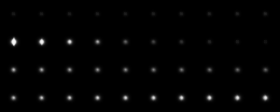
\includegraphics[width=\columnwidth]{assets/vae_interpolation.png}
    \caption{Linear interpolation between vectors in the latent space of the star variational autoencoder (\TODO{add this to the end of the report}).}
    \label{fig:vae_interpolation}
\end{figure}


\subsubsection{cDCGAN on Patches}
We found that a GAN that has to produce high resolution images is very hard to train. While our results from the DCGAN do follow the pattern from the cosmology data, the stars generally lack the necessary precise detail to make them look realistic. Hence, we explored a mixture of the straight-forward Adhoc with the DCGAN approach. We trained a smaller GAN on the $28\times28$ patches of the extracted stars. Since those patches resemble the MNIST \TODO{cite} data set in both spatial size and depth, we could simply adapt an existing architecture for our GAN \TODO{cite?}. For the generation of the high resolution data, the generator was fed some random latent code and the resulting star patches were put into the black background image in random fashion similar to the Adhoc method.

While this approach already produced quite convincing results, we decided to go one step further. We found that there were different kinds of stars inside the cosmology images; some very bright, some higher than broad, some very dark, some completely round. However, considering our large data set of around 15k star patches, most of them looked very similar, meaning they could potentially be divided into some small amount of individual classes. We trained a simple deep convolutional autoencoder (DCAE) on the star patches for 400 epochs. 
%We didn't have to worry about overfitting because we only wanted to cluster the same training data.
We then applied k-means clustering on each patch's latent code produced by the DCAE's encoder. That way, the stars were separated into five distinct classes. We did not have to worry about overfitting the DCAE, because it was only used on the data it was trained on.

Afterwards, we used the clustered data to train a conditional DCGAN (cDCGAN). Next to the image/latent code, the generator/discriminator are also fed the class label belonging to the star. To prevent the GAN from overfitting, we generated complete images every few epochs and included the best RF and CNN classifier models to score them. But we could not simply distribute the stars at random in the black background image, since this would not be an objective measurement for the generator score.
Hence, we measured the number of each star class on the given cosmology images and approximated it with a normal distribution bound to unsigned integers, because there cannot be a fraction number or a negative amount of stars in an image. We assumed the positioning of a star to be uniformly random. In order to be deterministic in the final result, we used a prototype cDCGAN model to distribute the stars following the specified distributions of number and positioning. Each time a set of 100 images was produced, the best RF and CNN models scored them. We repeated this process 2000 times and saved those random numbers that produced the highest score. With all the numbers saved, the next cDCGAN could then be trained with a deterministic validation procedure. 

The architecture of the cDCGAN was adopted from \TODO{cite} with the conditional property added. The architecture of the conditional generator can be seen in figure \ref{fig:cgen_arch}. It uses a total of \TODO{check} parameters. Figure \ref{fig:clustered_generated_stars} shows an generated example of the five different star classes. The discriminator uses a total of \TODO{check} parameters. Its architecture is illustrated in figure \ref{fig:cdis_arch}. The number of parameters is quite high and could have probably been lowered without loss of quality. However, since the generation of such small images is very stable, no architectural experiments were conducted. The cDCGAN was trained for 185 epochs, which lasted only about half an hour, from which around half the time was spent on validation. 
\begin{figure}
    \centering
    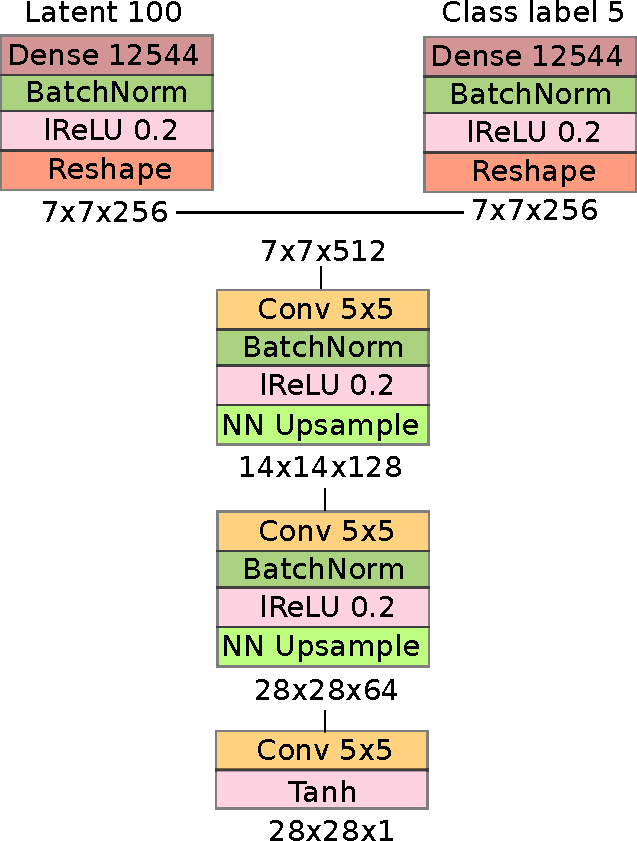
\includegraphics[width=0.6\columnwidth]{assets/cgen_arch.pdf}
    \caption{Illustration of the architecture of the conditional generator.}
    \label{fig:cgen_arch}
\end{figure}
\begin{figure}
    \centering
    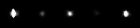
\includegraphics[width=\columnwidth]{assets/clustered_generated_stars.png}
    \caption{Example of the five different star classes generated by the cDCGAN.}
    \label{fig:clustered_generated_stars}
\end{figure}
\begin{figure}
    \centering
    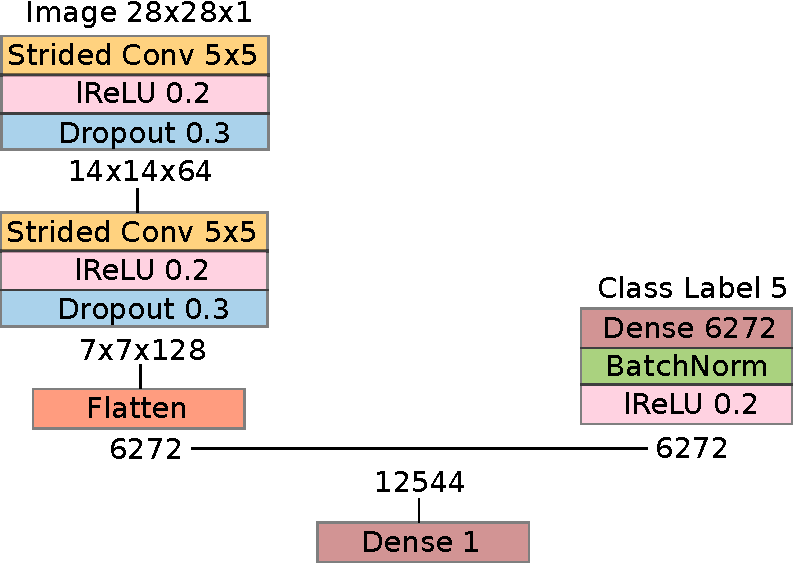
\includegraphics[width=0.75\columnwidth]{assets/cdis_arch.pdf}
    \caption{Illustration of the architecture of the conditional discriminator.}
    \label{fig:cdis_arch}
\end{figure}





\subsubsection{PixelCNN}
For the PixelCNN, we adopted the code from \TODO{cite} and replaced the MNIST with our own star patch data set. We evaluated a conditional and unconditional setting. The results looked strictly worse than those of the (c)DCGAN in both settings, so we did not bother to include the code any further into our existing project.



\section{Results}
\label{sec:results}
\subsection{Similarity Function Approximators}
Add short introduction to random forest.
For our random forest, a selection of different features was compared. All of these features are based on histograms of image properties. The results are shown in Table \ref{tab:RF}. \\

%\begin{table}[htbp]
%  \centering
%  \begin{tabular}[c]{|l||r|r|r|}
%    \hline
%        & \# features & MAE & STD \\
%    \hline
    
%    Pixel intensity + oriented gradients             &      90 + 36     &   0.177 & \\
%    Power spectral density             &    48       &  0.104 & \\
%    Power spectral density + ROI           &     48 + 48      &  0.086 & \\
%    \hline
%  \end{tabular}
%  \caption{Random Forest regression using different features.}
%  \label{tab:RF}
%\end{table}

\begin{table}\centering
\begin{tabular}{lrrr}
\toprule
& \# features & MAE & MAE \\
& & ~(pub.) & ~(priv.) \\
\midrule
Pixel intensity & 32 & 0.258 & 0.287  \\
Pixel intensity + oriented gradients & 32 + 36 & 0.177 & \\
Power spectral density & 48 & 0.104 & \\
Power spectral density + ROI & 48 + 48 & 0.086 & \\
\bottomrule
\end{tabular}
\caption{Random Forest regression using different features and the resulting Mean Absolute Error (MAE). \TODO{(Do we add the test split ratio here too?)}}\label{tab:RF}
\end{table}


We used histograms of image properties as features for random forest regression.

While the combination of a histogram of pixel intensities with a histogram of oriented gradients yielded better results, combining a histogram of the power spectral density with any other histogram led to a larger MAE in general. To better catch the distribution, we applied a log transformation. We tried to get better accuracy by filtering out certain angles as well as high or low frequencies. This is referred to as ROI. The number of bins was determined empirically. The range of the histogram was set according to mean and standard deviation of the distribution of the underlying data as well as according to minimum and maximum value values occuring in the data.


\begin{table}[htbp]
  \centering
  \begin{tabular}[c]{|l||r|r||r|r|}
    \hline
    Approximator    & Local MAE & STD   & Kaggle Pub.       & Kaggle Priv.\\ % kaggle descriptions
    \hline
    SRF             &           &       & 0.31661           & 0.31252\\ % With histogram fix
    CNN             &           &       & 0.16792           & 0.18781\\ % fft_4convs_8features_MAE
    ARF             &           &       & \textbf{0.09542}  & \textbf{0.10463}\\ % last one
    \hline
  \end{tabular}
  \caption{Mean Absolute Error (MAE) and Standard Deviation (STD), public Kaggle score and private Kaggle score for our various similarity function approximators.}
  \label{tab:SFA_MSS}
\end{table}

\begin{table}[htbp]
  \centering
  \begin{tabular}[c]{|l||r|r|}
    \hline
    Approximator    & Training time     & Scoring time \\
    \hline
    SRF             &                   &       \\
    CNN             & 24h               &       \\
    ARF             &                   &       \\
    \hline
  \end{tabular}
  \caption{Training and generation time for our various similarity function approximators.}
  \label{tab:SFA_time}
\end{table}


\subsection{Generators}
\begin{table}[htbp]
  \centering
  \begin{tabular}[c]{|l||r|r||r|r|}
    \hline
    Generator   & ARF MSS       & ARF STD   & CNN MSS       & CNN STD \\
    \hline
    AG          & 1.728         &           & 1.437         &  \\
    cDCGAN      & \textbf{3.044}& 1.088     & \textbf{2.613}& 0.886 \\
    VAE         & 1.723         &           & 2.026         &  \\
    %PixelCNN    &               &           &               &  \\
    \hline
  \end{tabular}
  \caption{Mean Similarity Score (MSS) and Standard Deviation (STD) as measured on the ARF and the CNN for our various generators. \TODO{We probably need to recalculate these}}
  \label{tab:gen_MSS}
\end{table}

\begin{table}[htbp]
  \centering
  \begin{tabular}[c]{|l||r|r|}
    \hline
    Generator   & Training time & Generation time \\
    \hline
    AG          &  -            &       \\
    cDCGAN      &               &       \\
    VAE         &               &       \\
    %PixelCNN    &               &       \\
    \hline
  \end{tabular}
  \caption{Training and generation time for our various generators.}
  \label{tab:gen_time}
\end{table}

To evaluate our generators we used our two best similarity function approximators, i.e. our ARF and CNN, to calculate the mean similarity score of the images. We chose not to train and use a conventional classifier to evaluate the generated images, as the Kaggle competition states that the images will be scored according to their mean similarity to a prototypical cosmology image. As such we decided to use the same evaluation process.
\TODO{TODO}



\section{Discussion}
\TODO{TODO}

\section{Summary}
By selectively extracting the most important features from images and learning to generate only these we achieved generated images superior than if the generative model learns to generate the image as a whole. This is judged by our similarity scorers.
\TODO{TODO}



\section*{Acknowledgements}
We would like to thank the assistants of the Computational Intelligence Lab for all their support and invariably fast replies to all our questions.


\bibliographystyle{IEEEtran}
\bibliography{cil_report}
\end{document}
